\documentclass[11pt,a4paper]{article}
\usepackage[utf8]{inputenc}
\usepackage{amsmath}
\usepackage{amsfonts}
\usepackage{amssymb}
\usepackage{graphicx}
\usepackage{booktabs}
\usepackage[left=2cm,right=2cm,top=2cm,bottom=2cm]{geometry}
\usepackage{authblk}
\title{\bf DEZSYS02 - DISTRIBUTED DATABASES}
\author{Janeczek Christian, Mair Wolfgang} 
\affil{IT Department TGM, Vienna}
\date{\today{}, Vienna}

\begin{document}

\maketitle
\newpage
\tableofcontents
\newpage

\section{Task Description}
\textbf{\underline{DEZSYS02 - VERTEILTE DATENBANKEN}}

\subsection{Introduction}
Es soll eine Verteilte Datenbank mit Oracle XE realisiert werden. Die Hauptaufgabe ist esherauszufinden wie man eine verteilte Datenbank erstellt. Die einzige Informationsquelle ist das weite Netz, allem voran die Oracle Dokumentation Site. Der komplette Datenbankentwurf für ein
verteiltes Oracle-DBS soll erstellt werden. Zu verwenden ist dabei eine geeignete
Fragmentierungsmethode! Die einzelnen Schritte sind zu dokumentieren, und Abfragen
durchzuführen, die eine Connection auf die verteilte Instanz nötig machen!

\subsection{Requirements}
Die MensaAustria plant die Erstellung einer Datenbank zur Vereinfachung der Arbeitsabläufe. Dabei
ist zu beachten, dass jede Universität ihre eigene Verwaltung bekommt, jedoch von einer Stelle
geleitet wird.
Eine Speise hat eine eindeutige Nummer, einen Namen und einen Typ (Vorspeise, Hauptspeise,
Nachspeise). Eine Speise besteht aus mehreren Zutaten, wobei die Menge der einzelnen Zutaten
gespeichert werden muss.
Eine Zutat hat eine eindeutige Nummer, einen Namen, eine Einheit (kg, Liter, etc.), einen Preis pro
Einheit und einen bzw. mehrere Lieferanten, von denen die Adresse und eine eindeutige
UIDNummer bekannt sind. Weiters wird die Kundennummer der Mensa beim jeweiligen Lieferanten
vermerkt. Der Lagerbestand wird ebenfalls modelliert. Dazu sind von jeder Zutat die Anzahl der
Einheiten, die momentan vorrätig sind, bekannt. Wenn eine Zutat nicht mehr vorrätig ist, so wird der
Bestand auf 0 gesetzt.
Im Falle einer Bestellung werden ein bzw. mehrere Zutaten bei einem bestimmten Lieferanten
bestellt. Die Bestellung hat eine eindeutige Bestellnummer, ein Bestelldatum, ein voraussichtliches
Lieferdatum. Die einzelnen Zutaten sind die Bestellposten, die eine pro Bestellung eindeutige
Nummer haben, und bei denen die bestellte Menge und der verhandelte Preis gespeichert werden.
Zu jeder Bestellung gibt es nach erfolgter Lieferung eine Rechnung, die verbucht werden muss.
Rechnungen beziehen sich auf genau eine Bestellung. Dabei wird die eindeutige Rechnungsnummer,
die Bankverbindung und die Rechnungssumme gespeichert, wobei letztere vom Bestellpreis
differieren kann, wenn ein Skonto anfällt.
Ein Menü hat einen eindeutigen Namen, einen Preis und es ist gespeichert, aus welchen
(verschiedenen) Speisen ein Menü besteht. Eine Speise kann selbstverständlich in mehreren Menüs
vorkommen.
Um eine zu große Eintönigkeit in der Menüabfolge zu vermeiden, wird weiters gespeichert, an
welchen Tagen welche Menüs serviert wurden. An jedem Tag werden genau drei Menüs serviert.

\newpage
\section{Technology}
\subsection{OracleXE}
OracleXE is an application which provides you with a database. You can also create

\newpage
\section{Design Consideration}
\subsection{Creating an Entity-Relationship-Diagram}
The first task would be to create an Entity-Relationship-Diagram to begin with. From this point on out we are able to discuss our current design concept. The next step would be to implement the whole idea into the already downloaded OracleXE Virtual Machine. But before that, the second task has to be fulfilled: you know it: Creating a Relational Model.
\subsection{Creating a Relational Model}
The creation of the Relational-Model had to be done simultaneously to the creation of the ER-Diagram to save as much time humanly possible. The underline command will be very useful here to differ between Primary Keys and Foreign Keys. Creating the Relational Model will be an easy task, because we have direct intercommunication with each person working on this very application.
\subsection{Implementing the whole concept in OracleXE}
\subsubsection{Configuring OracleXE}
Getting the OracleXE Virtual Machine and managing the whole configuration. 
\subsection{Working with SQL Developer}
We will work with SQL Developer and try to meet the requirements in the task description. The must-have task would be to convert the created concept of our CREATE SCRIPT into the SQL Developer solution. The task of creating specific inserts must not be forgotten. After that follows the creation of a second database with different INSERT values. Those two databases now have to be connected with some kind of Linker to prove the whole functionality of Distributed Databases.

\newpage
\section{Apportionment of work with effort estimation}

\textbf{Janeczek:} \\ \\
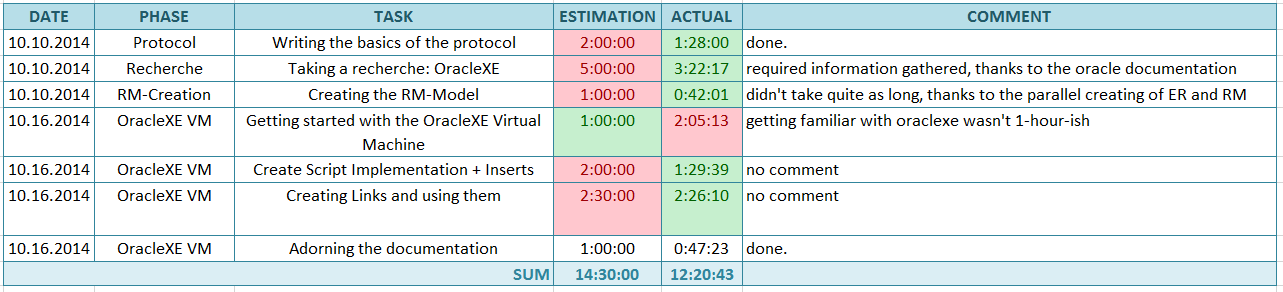
\includegraphics{wh-chris}
\textbf{Mair:} \\ \\
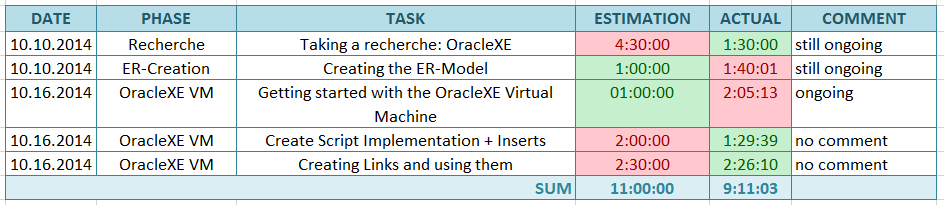
\includegraphics{wh-wolfi} \\ \\
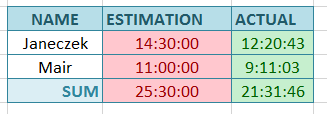
\includegraphics{wh-sum}

\newpage
\section{Task Execution}
\subsection{Creating an ER-Diagram}
The Entity-Relation-Diagram was successfully created.

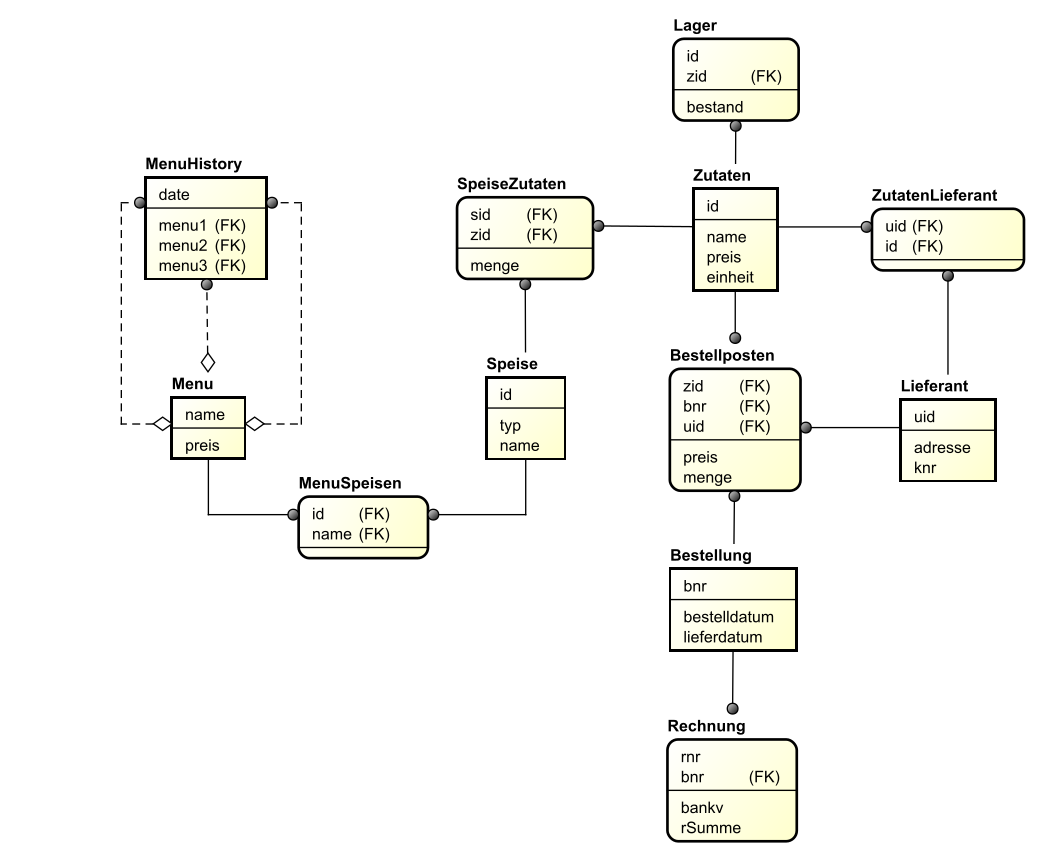
\includegraphics[scale=0.5]{dist-db-ERD}

\subsection{Creating a Relational Model}
The Relational Model was successfully created. \\ \\ MenuHistory(\underline{date}, Menu.name1, Menu.name2, Menu.name3) 3 meals per day \\
Menu(\underline{name}, preis) \\
MenuSpeisen(\underline{Speise.id}, \underline{Menu.name}) \\
Speise(\underline{id}, typ, name) \\
SpeiseZutaten(\underline{Speise.id}, \underline{Zutaten.id}, menge) \\
Zutaten(\underline{id}, name, preis, einheit) \\
ZutatenLieferant(\underline{Lieferant.uid}, \underline{Zutaten.id}) \\
Lieferant(\underline{uid}, adresse, knr) \\
Lager(\underline{id}, \underline{Zutaten.id}, bestand) \\
Bestellposten(\underline{Zutaten.id}, \underline{Bestellung.nr}, \underline{Lieferant.uid}, preis, menge) \\
Bestellung(\underline{bnr}, bestelldatum, lieferdatum) \\
Rechnung(\underline{rnr}, \underline{Bestellung.bnr}, bankv, rSumme) \\
\newpage
\subsection{Configuring OracleXE}
First of all, we had to get the Virtual Machine for OracleXE. This very Virtual Machine had already configured a functional OracleXE environment to work with. In this particular case we chose the password 'oracle'. So the login has got the following credentials: \\ \\ \textbf{username: system} \\ \textbf{password: oracle}
\subsection{Creating a new Database User}
The next step would be to create a new database user, baptised under the name 'janemair'. Put in the following command: \\ \\ \textbf{create user janemair identified by schueler;}
\subsection{Granting Privileges to 'janemair'}
As we know it from other Database-Management-System like postgreSQL and mySQL, we have to grant the newly created user some of the most important privileges. This is achieved by the already known command: \\ \\ \textbf{grant all privileges to janemair;}
\subsection{Installing SQL Developer}
To install and start SQL Developer use the following link referenced as: [1...http://www.oracle.com/technetwork/developer-tools/sql-developer/]
Just double-click the downloaded software and the package will be installed automatically.
\subsection{Creating new connections}
After SQL Developer was installed, the next thing to do is to create a connection, which needs the following information:
\begin{itemize}
	\item name of the connection
	\item username
	\item password
	\item type of the connection
	\item role
	\item hostname
	\item port
	\item name of the database (also known as SID)
	\item optionally: authentification configuration 
\end{itemize}
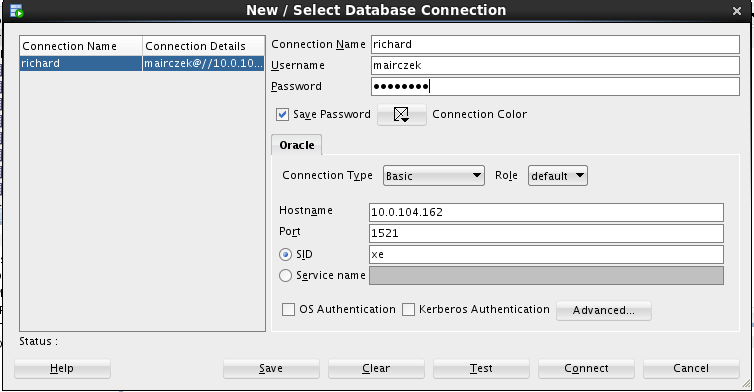
\includegraphics{richard-prop}

\subsection{Implementing the CREATE SCRIPT}
Thanks to useful Astah we are able to export a .sql CREATE SCRIPT from our ER-Diagram and import it directly to SQL Developer. All these beautiful tables and dependencies will be created automatically.
\subsection{Inserting Data}
The next step is to insert useful data into our database. This can be done either way:
\begin{itemize}
	\item Adding some INSERT lines in the .sql file, which has been imported and importing it again.
	\item INSERTING data via the most confusing GUI we have ever seen.
\end{itemize}
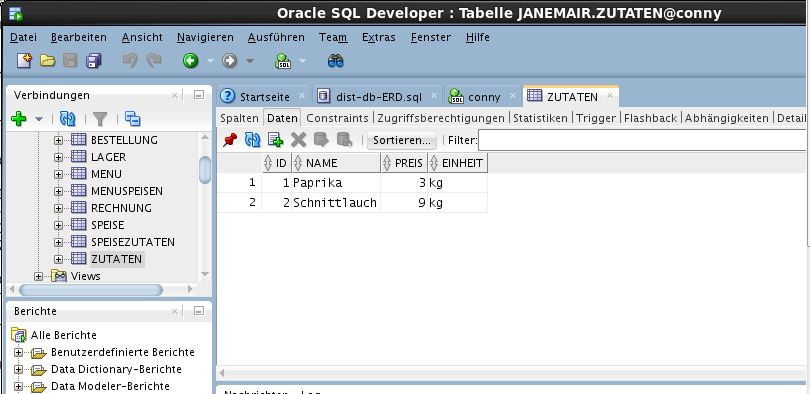
\includegraphics{DataMair}
\subsection{Creating another Database with different INSERTs}
After finally filling the database with data, we have yet to create a second database with different data but the struct of the db remains the same. \\ \\
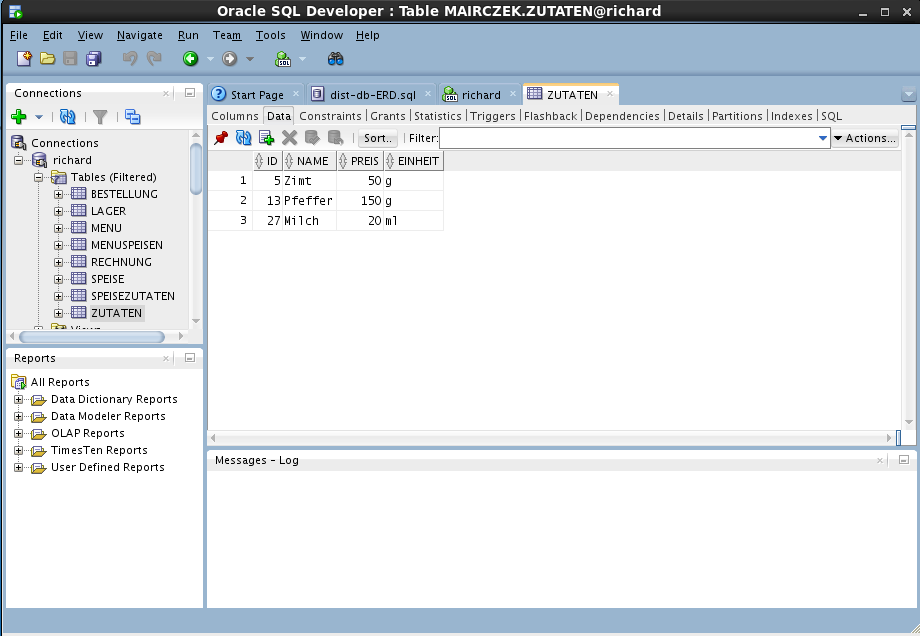
\includegraphics{richard}
\subsection{Linking the created Databases together}
To create a link which is able to get the data from another database you will need this code:\\ \\
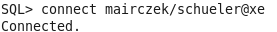
\includegraphics{connected} \\ \\
CREATE PUBLIC DATABASE LINK yada
CONNECT TO janemair IDENTIFIED BY password
USING '//192.168.43.242:1521/xe';\\ \\
"xe" would be the name of janemair's database \\ \\
\newpage
You can use this code then with the following select:\\

SELECT * FROM zutaten@yada;\\

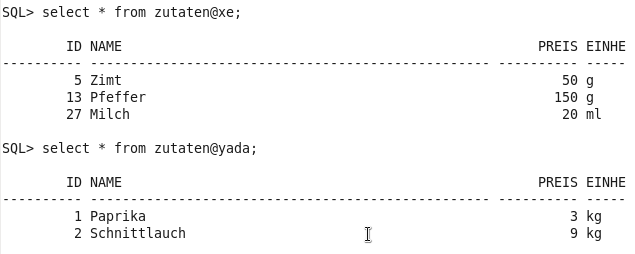
\includegraphics{selects} \\ \\
\bf ATTENTION: You have to check your network configuration some connections (as an example the TGM network) is blocking such features. \\
\newpage

\section{Test Report}
\newpage

\bibliographystyle{IEEEtran}
\bibliography{References}

\end{document}
